\chapter{Technologies involved}
\label{chapter:near-term}

 In this chapter we discuss technologies used for performing research presented in this work.
 First, we discuss quantum annealing, a quantum computation paradigm witnessing rapid development in recent years. The second discussed technology, Nvidia CUDA, is present on the market for well over a decade, yet each and every iteration of GPUs brings to the table new functionalities and performance improvements. 


\section{Adiabatic quantum computation and quantum annealing}
One of the possible alternatives to the standard gate model is adiabatic quantum computation which relies on adiabatic quantum theorem \cite{born}. Informally, the theorem states that if the physical system starting from its instantenous ground state is driven slowly enough, the evolution follows hamiltonian and the system stays in the instantenous ground state. Adiabatic quantum computing might be realized in a form of quantum annealing. In this metaheuristics, a goal is to minimize value of some target function $f$. In order to do so, one first has to find some Ising hamiltonian $H$ whose ground state encodes the optimal solution to the problem. Then, the system is prepared in a ground state of some initial, simpler hamiltonian $H_0$. After that. the system is slowly perturbed in such a way that its hamiltonian changes from $H_0$ to $H$, i.e. the evolution of the system is governed by the following hamiltonian $H_\text{total}$
\begin{equation}
    \label{eq:aqc}
    {H}_\text{total}(s) = a(s) {H}_0 + b(s){H}, \quad s \in [0, \tau]
\end{equation}
where $a(\tau) = b(0) = 0, \; a(0) = b(\tau) = 1$, and $a$ and $b$ are decreasing and increasing functions respectively.
By adiabatic quantum theorem, if the evolution described by the equation \eqref{eq:aqc} is slow enough, the system will stay in ground state of ${H}_\text{total}(s)$ for every $s \in [0, \tau]$. In particular, after reaching $s=\tau$, i.e. when $H_\text{total} = H$, the state of the system should encode an optimal solution to target optimization problem.


\subsection{D-Wave quantum annealers}

The first commercially available quantum annealer was introduced by D-Wave company in 2011. At the time of writing, the newest series of D-Wave annealers is The Advantage System utilizing chip with at least 5000 qubits. These novel devices deomnstrate a significant improvement over previous 2000Q generation, which used at most 2048 qubit chip with sparser connectivity. Since most research utilizing quantum annealers in this work was conducted using 2000Q devices, in what follows we mostly limit our attention to this specific devices.

\begin{figure}[h]
    \centering
    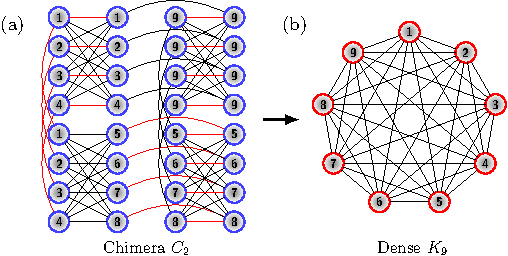
\includegraphics[width=\textwidth]{figures/chimera.pdf}
    \caption{\textbf{a.} Example of Chimera topology. Graph presented here consists of $2 \times 2$ grid of unit cells (hence $C_2$ name). Note the sparse connectivity of the presented graph as compared to the full graph with the same number of nodes. \textbf{b.} Full $K_9$ graph embedded in Chimera graph from \textbf{a.}. The nodes are labelled with numbers corresponding to groups of logical qubits they were constructed from.}
    \label{fig:chimera}
\end{figure}


\subsection{Annealer topologies and minor embeddings}

The Ising model described in previous chapter allows arbitrary interactions between spins. However, this is often not the case with physical devices like quantum annealers. For instance, in D-Wave devices spins are arranged into a specific \emph{topology} with limited connectivity. Thus, the possible graph on which the optimization problems can be defined is much sparser than the complete $K_{N}$ graph. Spins in 2000Q devices are arranged in the so called \emph{Chimera} topology depicted in figure \ref{fig:chimera}. The Chimera graph can be thought of as a $n \times m$ lattice of unit cells, where each cell is a complete bipartite $K_{4,4}$. Qubits are also connected to two qubits in neighbouring cells via external couplers (unless they reside on the border or a corner of the lattice), resulting in at most total 6 connections per qubit. Straightforward calculation shows that Chimera graph has total of $16mn + 4(m-1)n + 4(n-1)m$ edges.

The new Advantage system uses \emph{Pegasus} topology, which increases maximum degree of vertex in the graph to 15. For the details of this topology we refer interested reader to \cite{boothby}.


\section{Nvidia CUDA}
History of specialized hardware for manipulating graphics ranges as far as to 1970s. Initially these devices, that later became known as Graphics Processing Units (GPU), offered limited functionalities. Increasing demand for performance in gaming industry and professional graphics processing drove the evolution of GPUs, which quickly became highly sophisticated devices supporting advanced 2D and 3D image manipulation. Performing such arithmetically intensive operations requires enormous computational power, and it was only the matter of time until it was realised that the power of these devices can be harnessed for general purpose computations (so called GPGPU - General Purpose computing on GPU). 

Early efforts in development of GPGPU required framing of computational problem in terms of operations performed on graphical primitives, as this was the only way for using specialized API of GPUs. This changed with the development of devices and toolkits that supported operations needed for general purpose computations out of the box. Notably, in 2007 Nvidia introduced its massively parallel CUDA architecture.

\subsection{Differences between CPU and GPU}
Principles behind operation of CUDA-enabled devices are fundamentally different than the ones governing execution of program on traditional CPU-only architecture. In current x86 based computers, CPU runs given sequence of instructions (so called thread of execution) using one of its cores. Such processor is the ''brain'' of a computer, and it can perform a wide variety of tasks ranging from arithmetic operations, through accessing system's RAM, to performing IO operations and controlling other components of the system. Typical CPUs are optimized for sequential execution, and as such are usually equipped with moderate (as compared to the GPUs) number of high-performance cores. 

On the other hand, GPUs are more specialized. They are well suited for performing a large number of arithmetic operations and accessing memory in parallel. They typically have more cores than a traditional CPU (with even modern commodity GPUs boasting thousands of them). Although those cores are less performant than their CPU counterparts and support much narrower set of operations, their large number combined with fast memory access gives modern GPUs advantage over CPUs in multiple areas.

\subsection{Processing flow on CUDA}
Considering the architectural differences between CPUs and GPUs, it is hardly surprising that both of these types of devices are programmed quite differently. The first major difference is that GPUs cannot operate on their own and are themselves controlled by CPU. This is why CUDA is a type of \emph{heterogenous} architectures (as opposed to CPU-only \emph{homogenous} architectures). The processing flow on CUDA is summarized in Figure \ref{fig:cuda_flow}.

\begin{figure}[ht]
    \centering
    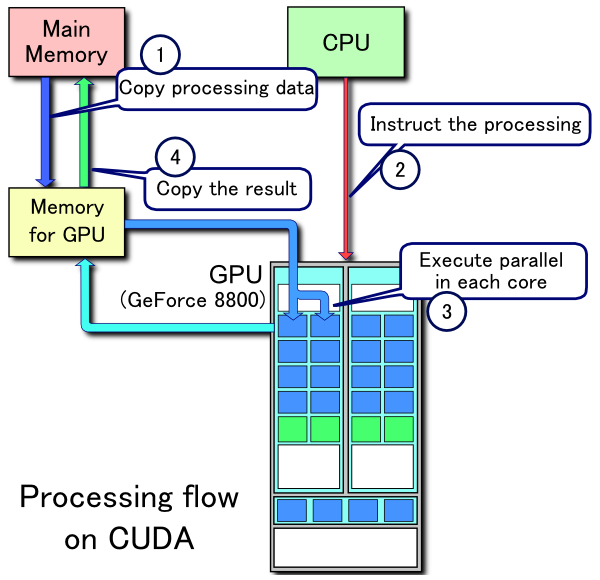
\includegraphics[width=0.7\textwidth]{figures/CUDA_processing_flow_(En).png}
    \caption{{\protect\todo[inline]{Important: this figure is only here temporarily, I will prepare my own graph once the text is done.}} Processing flow on CUDA. The CPU sends input data to GPU memory, and launches computational kernel. The kernel's code is executed, in parallel, using GPU. Once the execution is done, results are copied form GPU memory to system's RAM.}
    \label{fig:cuda_flow}
\end{figure}

Programs run on GPU are organized in \emph{kernels}. For the most part kernels might be viewed as functions or subroutines (which is indeed how they are implemented) that don't have a return value. On a CPU, such function would be executed by some core as a part of a thread. In CUDA however, the very same kernel is executed by multiple threads. Executing a kernel requires specifying a \emph{grid} that will be used for running it. A grid can be 1, 2 or 3 dimensional and is itself divided into blocks. Each block is in turn also organized in 1, 2, or 3 dimensional structure of threads (the same for every block in the grid). Schematic view of a two-dimensional grid is presented on Figure \ref{fig:cuda_grid}.

\begin{figure}[ht]
    \centering
    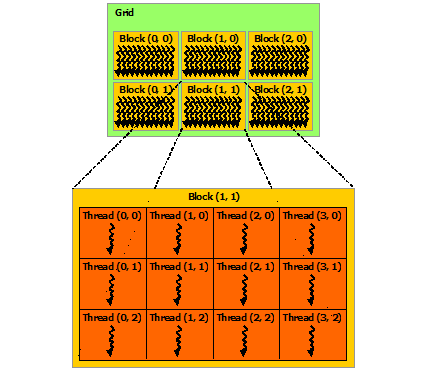
\includegraphics[width=0.8\textwidth]{figures/grid-of-thread-blocks.png}
    \caption{{\protect \todo[inline]{This is also a temporary figure...}} A schematic view of an example two-dimensional CUDA grid. Presented here is a 2 $\times$ 3 grid of 3 $\times$ 4 blocks.}
    \label{fig:cuda_grid}
\end{figure}

As already mentioned, each thread in the grid executes \emph{precisely the same} kernel. It might therefore seem surprising that nevertheless they are able to access different parts of memory. This is possible, because each thread is identified by its indices in both the grid and the block. Those indices can be used e.g. for computing offsets in arrays that are being processed. A more sophisticated use of thread and block indices will be exemplified in chapter \ref{chapter:bruteforce}.

\subsection{Programming environment}
CUDA devices can be programmed directly using either C/C++ or Fortran. The C/C++ code can be compiled using Nvidia's nvcc compiler, shipped out of the box with CUDA toolkit, while using Fortran requires installing its third-party distribution (e.g. PG Fortran developed by Portland Group). Giving a comprehensive walkthrough of using either C/C++ or Fortran with CUDA is well beyond the scope of this thesis, but for the sake of completeness we present a short example of CUDA Fortran code in listing \ref{lst:cuda_fortran} \todo{Note to self: remember to either replace it with my own example or cite the source (CUDA Fortran documentatoin)}. 

\begin{lstlisting}[
    language=Fortran,
    label=lst:cuda_fortran,
    captionpos=b,
    caption={Example code in CUDA Fortran. Presented here are an example kernel performing saxpy operation together with a host subroutine that uses it.},
    frame=tlrb,
    aboveskip=2em,
    belowskip=2em
]{fortran}
! Kernel definition
attributes(global) subroutine ksaxpy( n, a, x, y )
   real, dimension(*) :: x,y
   real, value :: a
   integer, value :: n, i
   i = (blockidx%x-1) * blockdim%x + threadidx%x
   if( i <= n ) y(i) = a * x(i) + y(i)
end subroutine

! Host subroutine
subroutine solve( n, a, x, y )
   real, device, dimension(*) :: x, y
   real :: a
   integer :: n
   ! call the kernel
   call ksaxpy<<<n/64, 64>>>( n, a, x, y )
end subroutine
\end{lstlisting}

Along the nvcc compiler, the CUDA toolkit contains several, more specialized libraries. Among others, those include:
\begin{itemize}
    \item cuBLAS -- CUDA Basic Linear Algebra Subroutines library,
    \item cuFFT -- CUDA Fast Fourier Transform library,
    \item cuRAND -- CUDA Random Number Generation library,
    \item cuSPARSE -- CUDA library for manipulating sparse matrices.
\end{itemize}
For many high-level languages, there exist third-party wrappers enabling use of CUDA (e.g. PyCuda for Python).



%%% Local Variables:
%%% mode: latex
%%% TeX-master: "../main"
%%% End:
